
  \documentclass{lxaiproposal}
  \usepackage{hyperref}
  
  %   \usepackage[english,french]{babel}   % "babel.sty" + "french.sty"
     \usepackage[english]{babel}   % "babel.sty" + "french.sty"
     
  % \usepackage[english,francais]{babel} % "babel.sty"
  % \usepackage{french}                  % "french.sty"
    \usepackage{times}			% ajout times le 30 mai 2003
   
  \usepackage{epsfig}
  \usepackage{graphicx}
  \usepackage{amsmath}
  \usepackage{amssymb}
   \usepackage{booktabs}
   \usepackage{multirow}
  \usepackage{pifont}
  \usepackage{caption}
  \usepackage{subcaption}
  
  
  
  \usepackage{array}
  \usepackage{color}
  \usepackage{colortbl}
  
  \usepackage{pifont}
  \usepackage{amssymb}
  \usepackage{latexsym}
  
  \usepackage{booktabs}
  
  %% --------------------------------------------------------------
  %% FONTS CODING ?
  % \usepackage[OT1]{fontenc} % Old fonts
  % \usepackage[T1]{fontenc}  % New fonts (preferred)
  %% ==============================================================
  
  \title{Improving Elevator System using RFID and Emergency Stuck System}
  
  \author{\coord{Shajaratul}{Yakin}{1} \\
         \coord{Sudipta Kumar}{Das}{2}\\
         \coord{Parvez, Md. Najmus Shakib Khasru}{}{3} \\
         \coord{Snahasish}{Dey}{4}\\
         \coord{Mitu Rani}{Ghosh}{5} \\
         \coord{Nousheen}{Jahan}{6} \\
         \coord{Badhon}{Sutrudhar}{7}
        }
  
  \address{\affil{1}{American International University-Bangladesh, 408/1, Kuratoli, 1229}}
  
  %% If all authors have the same address %%%%%%%%%%%%%%%%%%%%%%%%%%%%%%%%%%%%%%%
  %                                                                             %
  %   \auteur{\coord{Michel}{Dupont}{},                                         %
  %           \coord{Marcel}{Dupond}{},                                         %
  %           \coord{Michelle}{Durand}{},                                       %
  %           \coord{Marcelle}{Durand}{}}                                       %
  %                                                                             %
  %   \adress{\affil{}{Laboratoire Traitement des Signaux et des Images \\      %
  %     1 rue de la Science, BP 00000, 99999 Nouvelleville Cedex 00, France}}   %
  %                                                                             %
  %                                                                             %
  %%%%%%%%%%%%%%%%%%%%%%%%%%%%%%%%%%%%%%%%%%%%%%%%%%%%%%%%%%%%%%%%%%%%%%%%%%%%%%%
  
%   \email{PI email, CO-PI email}
  
%   \englishabstract{}
  
\begin{document}
\maketitle
%
\section{Background and Motivation}
\vspace*{-3mm}

Elevators are a type of modern transportation that are frequently used to transfer people or things vertically in tall buildings like hotels, retail malls, and offices. The elevator
control system's primary goals are to direct the elevator car to the target floor, cut travel time, and enforce the safe speed restriction\cite{r2}. ``Werner von Siemens", a German inventor,
introduced the electric motor with elevator technology in the 1800s after the invention of electricity. By 1903, this concept had developed into the gearless traction
electric elevator, making it feasible to construct structures with more than 100 stories and permanently altering the urban environment. \cite{r1}



% \section{Problem Statement}
% \vspace*{-3mm}

% You should describe Intellectual Merit \cite{r2}: The intellectual Merit criterion encompasses the potential to advance knowledge (Technical relevance for startups/NGOs, Scientific relevance for academic projects) as compared to related works.

% Discuss in a more focused manner how your AI project will solve the problem stated above and how you plan to build upon the state of the art.
% \textbf{(1-2 paragraphs)}


\section{Goals and Benefits of the Project}
\vspace*{-3mm}

Nowadays, elevators are using in everywhere. In every hospital, market, and office building there is some restricted elevator that is available for authorized persons only.
But sometimes unauthorized persons use that elevator. So, we are planning to modify the traditional elevator system using an RFID Card. Only authorized persons will have RFID
Cards without RFID cards elevator doors won't open. Which will keep the elevator more restricted. Also, we are planning to make the elevator more secure. If the elevator will
unattached from its wire, the elevator will fall down and people will die. So, we are planning to implement an Emergency Stuck system. When the elevator will fall down, it will
stuck there.
    {\vskip 1em}
After implementing these two systems, the elevator will be more secure and restricted. No unauthorized person will use the elevator. And the RFID system will also help disable person
for whom clicking buttons is not easy, can also easily use the elevator by their own. Also, if the elevator will fall down, the emergency stuck system will save the people. So,that
is the way the elevating system will be more upgraded and secured.


% \section{Expected Results and Impact}
% \vspace*{-3mm}

% Describe which impact and outcomes your project will have. For academic projects you can discuss in terms of human resources formation, development of any publicly available dataset, new capabilities, impact in larger projects, advance state-of-the-art knowledge, etc.
% \textbf{(1 page)}

\newpage %%%%%%%%%%%%%%%%%%%%%%%%%%%%%%%%%%%%%%%%%%%%%%%%%%%%%%%%%%%%%%%%%%%%%%%%%%%%%%%%%%%%%%% NEW PAGE HERE  

\section{Survey to develop a process for complex engineering problems considering cultural and societal factors }
\vspace*{-3mm}
% \begin{figure}[htbp]
%     \begin{center}
%         \fbox{\includegraphics*[width=8cm]{images/Q1.png}}
%         \caption{Article Search Result}
%     \end{center}
% \end{figure}
The survey questions are,
\begin{itemize}
    \item Do you know about RFID Cards?
          \begin{figure} [h!]
              \centering
              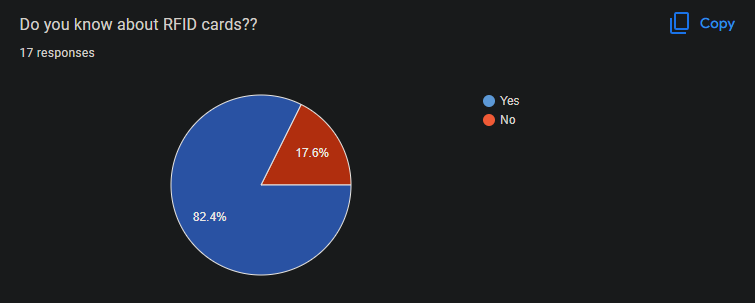
\includegraphics[width=1\linewidth]{images/Q1.png}
              \caption{Responses for question no 1}
              \label{fig:my-fig}
          \end{figure}
    \item Are you interested in using RFID Card in the elevator system?
          \begin{figure} [h!]
              \centering
              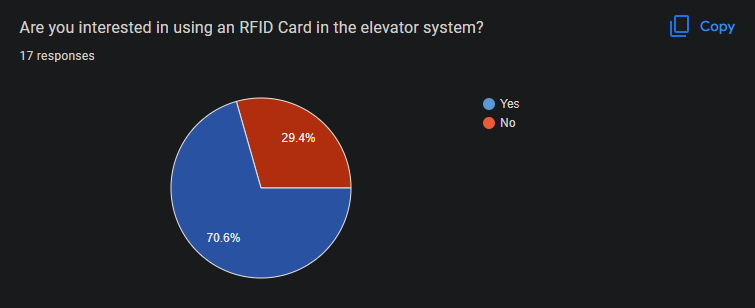
\includegraphics[width=1\linewidth]{images/Q2.png}
              \caption{Responses for question no 2}
              \label{fig:my-fig}
          \end{figure}

          \newpage %%%%%%%%%%%%%%%%%%%%%%%%%%%%%%%%%%%%%%%%%%%%%%%%%%%%%%%%%%%%%%%%%%%%%%%%%%%%%%%%%%%%%%% NEW PAGE HERE  

    \item Do you think that authorized life will be more secure with RFID Card validation?
          \begin{figure} [h!]
              \centering
              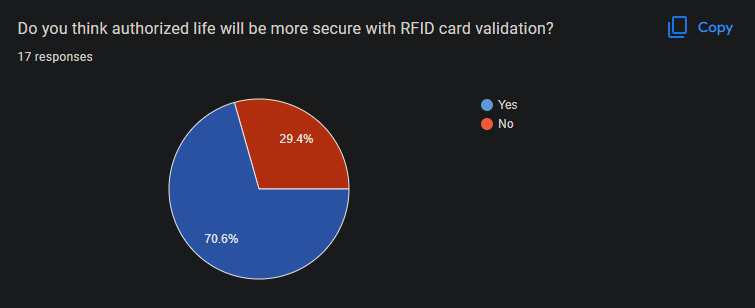
\includegraphics[width=1\linewidth]{images/Q3.png}
              \caption{Responses for question no 3}
              \label{fig:my-fig}
          \end{figure}
    \item Which one do you prefer?
          \begin{figure} [h!]
              \centering
              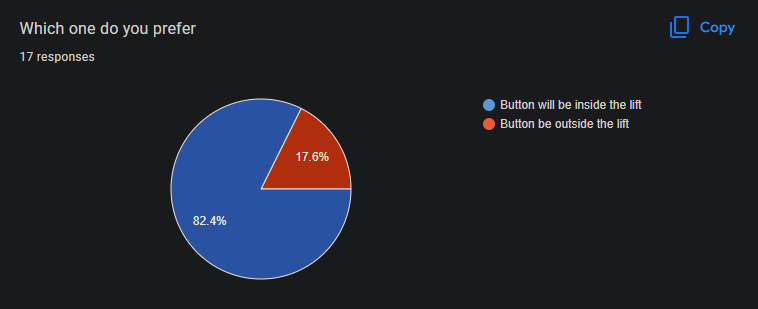
\includegraphics[width=1\linewidth]{images/Q4.png}
              \caption{Responses for question no 4}
              \label{fig:my-fig}
          \end{figure}
\end{itemize}


\section{Experimental Block Diagram}
\vspace*{-3mm}

\begin{figure} [h!]
    \centering
    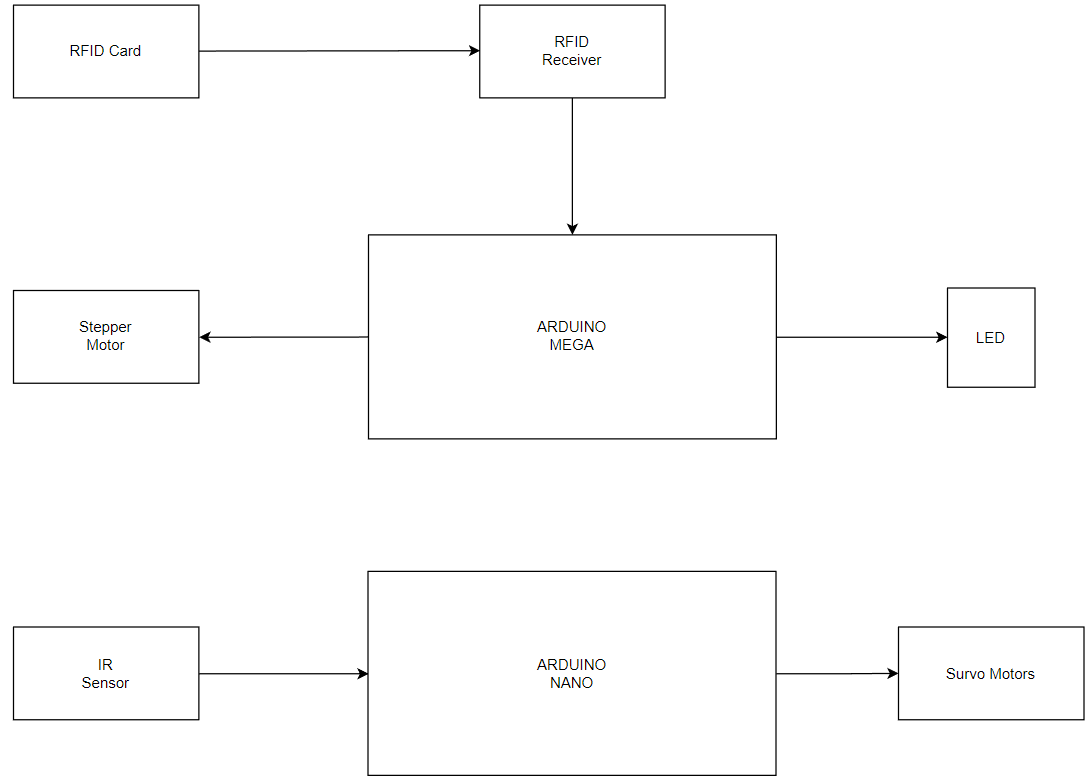
\includegraphics[width=1\linewidth]{images/Improving Elevator System Block Diagram.png}
    \caption{Improving Elevator System Block Diagram}
    \label{fig:my-fig}
\end{figure}

\newpage %%%%%%%%%%%%%%%%%%%%%%%%%%%%%%%%%%%%%%%%%%%%%%%%%%%%%%%%%%%%%%%%%%%%%%%%%%%%%%%%%%%%%%% NEW PAGE HERE  

\section{Project Timeline(Gantt Chart)}
\vspace*{-3mm}

\begin{figure} [h!]
    \centering
    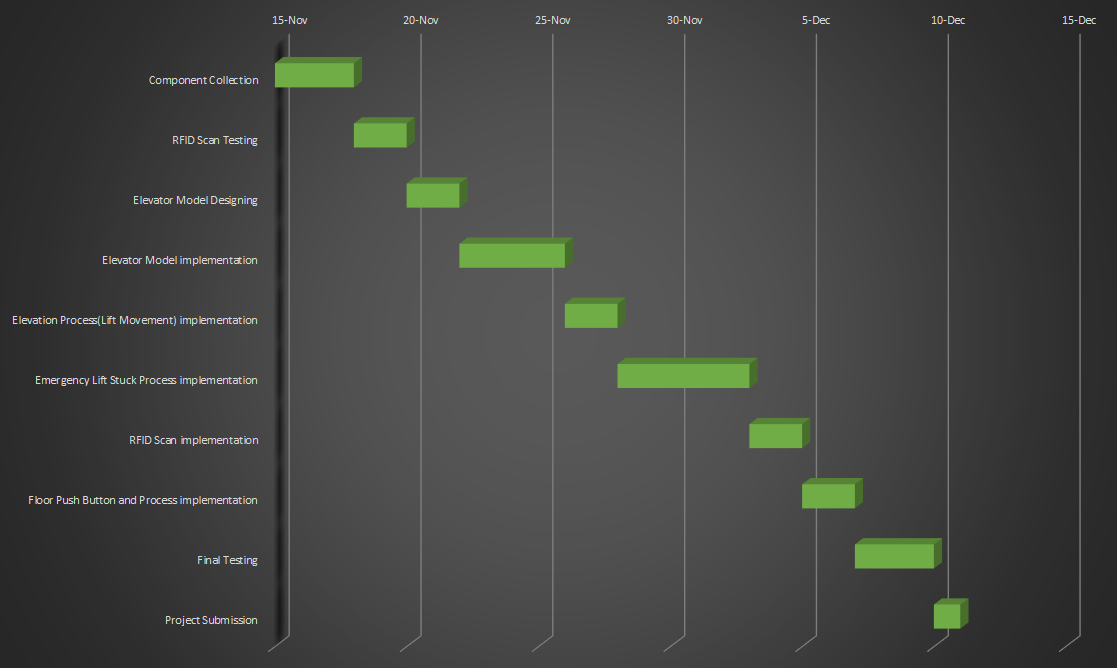
\includegraphics[width=1\linewidth]{images/GANN CHART.png}
    \caption{Gantt Chart}
    \label{fig:my-fig}
\end{figure}










\bibliographystyle{ieee_fullname}
\bibliography{references}

%\begin{thebibliography}{99}
%\end{thebibliography}

\end{document}




































% Please add the following required packages to your document preamble:
% \begin{table}[h!]
%     \centering
%     \caption{A typical table.}
%     \label{tab:my-table}
%     \begin{tabular}{@{}ccccc@{}}
%         \toprule
%         \textbf{Items/Cols} & \textbf{Col 1} & \textbf{Col 2} & \textbf{Col 3} & \textbf{Col 4} \\ \midrule
%         \textbf{Item 1}     & Value          & Value          & Value          & Value          \\
%         \textbf{Item 2}     & Value          & Value          & Value          & Value          \\
%         \textbf{Item 3}     & Value          & Value          & Value          & Value          \\ \bottomrule
%     \end{tabular}
% \end{table}

%\begin{figure} [h!]
%    \centering
%    \includegraphics[width=1\linewidth]{images/fig1.png}
%  \caption{A typical figure.}
%    \label{fig:my-fig}
%    \end{figure}
